\documentclass[runningheads,a4paper,fleqn]{llncs}

\usepackage{url}
\usepackage{amsmath}
\usepackage{amssymb}
\usepackage{alltt}
\usepackage{lineno}
\usepackage{graphicx}
\usepackage{subfigure}
\usepackage[normalem]{ulem}

\usepackage{tikz}
\usetikzlibrary{arrows,petri,topaths}
\usepackage{tkz-berge}

\begin{document}

\title{FlowArrays: Barrier-Free ParArrays}
\author{Tobias Schlatter\inst{1} \and Heather Miller\inst{2} \and
  Aleksandar Prokopec\inst{2} \and Philipp Haller\inst{2} \and Martin
  Odersky\inst{2}}

\authorrunning{Tobias Schlatter}

\institute{Student, EPFL \and Advisors, EPFL}

\graphicspath{{figs/}}

\newcommand{\plot}[1]{\input{../../benchmarks/flowArrays/plots/#1}}

\maketitle

\begin{abstract}
  In \cite{FP12} we proposed an unordered, barrier- and lock-free,
  parallel datastructure, the \texttt{FlowPools}. Attempts to implement a
  bigger application using \texttt{FlowPools}, showed that the lack of ordering
  is very limiting. \texttt{FlowArrays}, proposed by this report, do not have
  this limitation -- having a very similar structure than
  \texttt{ParArrays} \cite{collect11}, \texttt{FlowArrays} eliminate the need to block
  in between two monadic operations while exposing a very similar
  interface to the programmer.

  Benchmarks on operations for linear algebra have shown that the
  current implementation of \texttt{FlowArrays} performs comparable to
  \texttt{ParArrays}. Further, we will find that with the current storage model
  of \texttt{FlowArrays}, garbage collection takes considerably more time than
  actual calculation. We can show that
  the adaptions proposed later on in this report do significantly
  speed up the calculation and will lead to higher performance than
  \texttt{ParArrays}.
\end{abstract}

\section{Introduction}
% Stolen from \cite{FP12}
Multicore architectures have become ubiquitous -- even most mobile devices now
ship with multiple core processors. Yet parallel programming has yet to enter
the daily workflow of the mainstream developer. One significant obstacle is an
undesirable choice programmers must often face when solving a problem that
could greatly benefit from leveraging available parallelism. Either choose a
non-deterministic, but performant, data structure or programming model, or
sacrifice performance for the sake of clarity and correctness.

Programming models based on \emph{dataflow} \cite{Arvind89,CnC10} have the
potential to simplify parallel programming, since the resulting programs are
deterministic. Moreover, dataflow programs can be expressed more declaratively
than programs based on mainstream concurrency constructs, such as shared-memory 
threads and locks, as programmers are only required to specify data and
control dependencies. This allows one to reason sequentially about the
intended behavior of their program, meanwhile enabling the underlying
framework to effectively extract parallelism.

In an earlier paper \cite{FP12} we proposed \texttt{FlowPools}, a
deterministic, dataflow abstraction. Since they're unordered,
\texttt{FlowPools} have been
shown to be somewhat limited when it comes to implementing concrete
applications. This report presents \texttt{FlowArrays}, an immutable
dataflow structure very much like sequences with monadic
operations. Contrary to normal \texttt{Seqs} (or \texttt{ParArrays}
\cite{collect11}), \texttt{FlowArrays} have the characteristics of a
\emph{dataflow collection} -- i.e. they do not block in between
monadic operations until the calculation is complete, but do the
calculation asynchronously.

The dataflow in this programming model is implicit: The programmer can
use the known functional programming abstractions and only has to
make a special call when retrieving concrete results.

\texttt{FlowArrays} have been designed with the use case of linear
algebra operations in mind; hence, they are fixed-size and support
operations like \texttt{transpose} and \texttt{slice}.

First we give an overview of the general idea behind \texttt{FlowArrays} and
how exactly they try to improve on \texttt{ParArrays}. The section outlines the
basic concepts of how task splitting in \texttt{FlowArrays} is done. The next
section describes how \texttt{FlowArrays} are implemented in detail. The
evaluation section analyzes the performance of \texttt{FlowArrays} using vector
scalar products as a benchmark. In the conclusion, we will propose
improvements and future work.

Our contributions are the following:
\begin{enumerate}
\item The design and Scala~\cite{Odersky10} implementation of a
  \texttt{ParArray}-like, but non-blocking datastructure.
\item Benchmarks comparing \texttt{FlowArrays} to \texttt{ParArrays} with a focus on
  garbage collection overhead.
\item A proposition for significant speed increase due to reduced GC
  overhead.
\end{enumerate}

\section{Overview}
\label{sec:overview}

In this section we will first outline how \texttt{FlowArrays} strive to improve
on \texttt{ParArrays} from an abstract perspective. Then we will show some of
the difficulties that arise particularly with this approach.

\subsection{Barrier-Freedom}
\texttt{FlowArrays} are, unlike \texttt{ParArrays}, barrier-free. We will use a simple
example, a single \texttt{map} operation, to show how these two
datastructures differ.

Let's consider the following code for \texttt{ParArrays} and
\texttt{FlowArrays}. Fig.~\ref{fig:barrier-free} shows a schematic
illustration of what is going on.

\noindent
\begin{minipage}[t]{.5\textwidth}
\begin{alltt}
{\scriptsize
val pa1 = ParArray.tabulate(n)(x => x*x)
val pa2 = pa1.map(_ * 2)
}
\end{alltt}
\end{minipage}
\begin{minipage}[t]{.5\textwidth}
\begin{alltt}
{\scriptsize
val fa1 = FlowArray.tabulate(n)(x => x*x)
val fa2 = fa1.map(_ * 2)
}
\end{alltt}
\end{minipage}

In both cases, we first create a \texttt{Par/FlowArray} using
\texttt{tabulate}. Both Par- and \texttt{FlowArrays} will use exponential task
splitting \cite{collect11,cong08} to distribute the workload of
calculating the individual elements. The crucial difference between
\texttt{ParArrays} and \texttt{FlowArrays} starts here: with \texttt{ParArrays}, the call to
\texttt{tabulate} (and any other function for that matter) will only
return once every element has been calculated. In contrast, the call
to \texttt{tabulate} on \texttt{FlowArrays} will return immediately, yielding
an array whose elements are well-defined, but not yet calculated.

When calling \texttt{map} on the first \texttt{Par/FlowArray}, this difference
becomes even clearer: \texttt{ParArrays} will do the same thing as for
\texttt{tabulate}; split up the task of calculation and start right
away. \texttt{FlowArrays} however, will align the task blocks and start
calculating the elements once the elements on which the result depends have
been calculated (in our case the result of the \texttt{tabulate}). So,
contrary to \texttt{ParArrays}, \texttt{FlowArrays} are able to start subsequent
calculations partially, even if not all the elements of the original
array have been calculated.

\begin{figure}
  \centering
  \subfigure[\texttt{ParArray}] {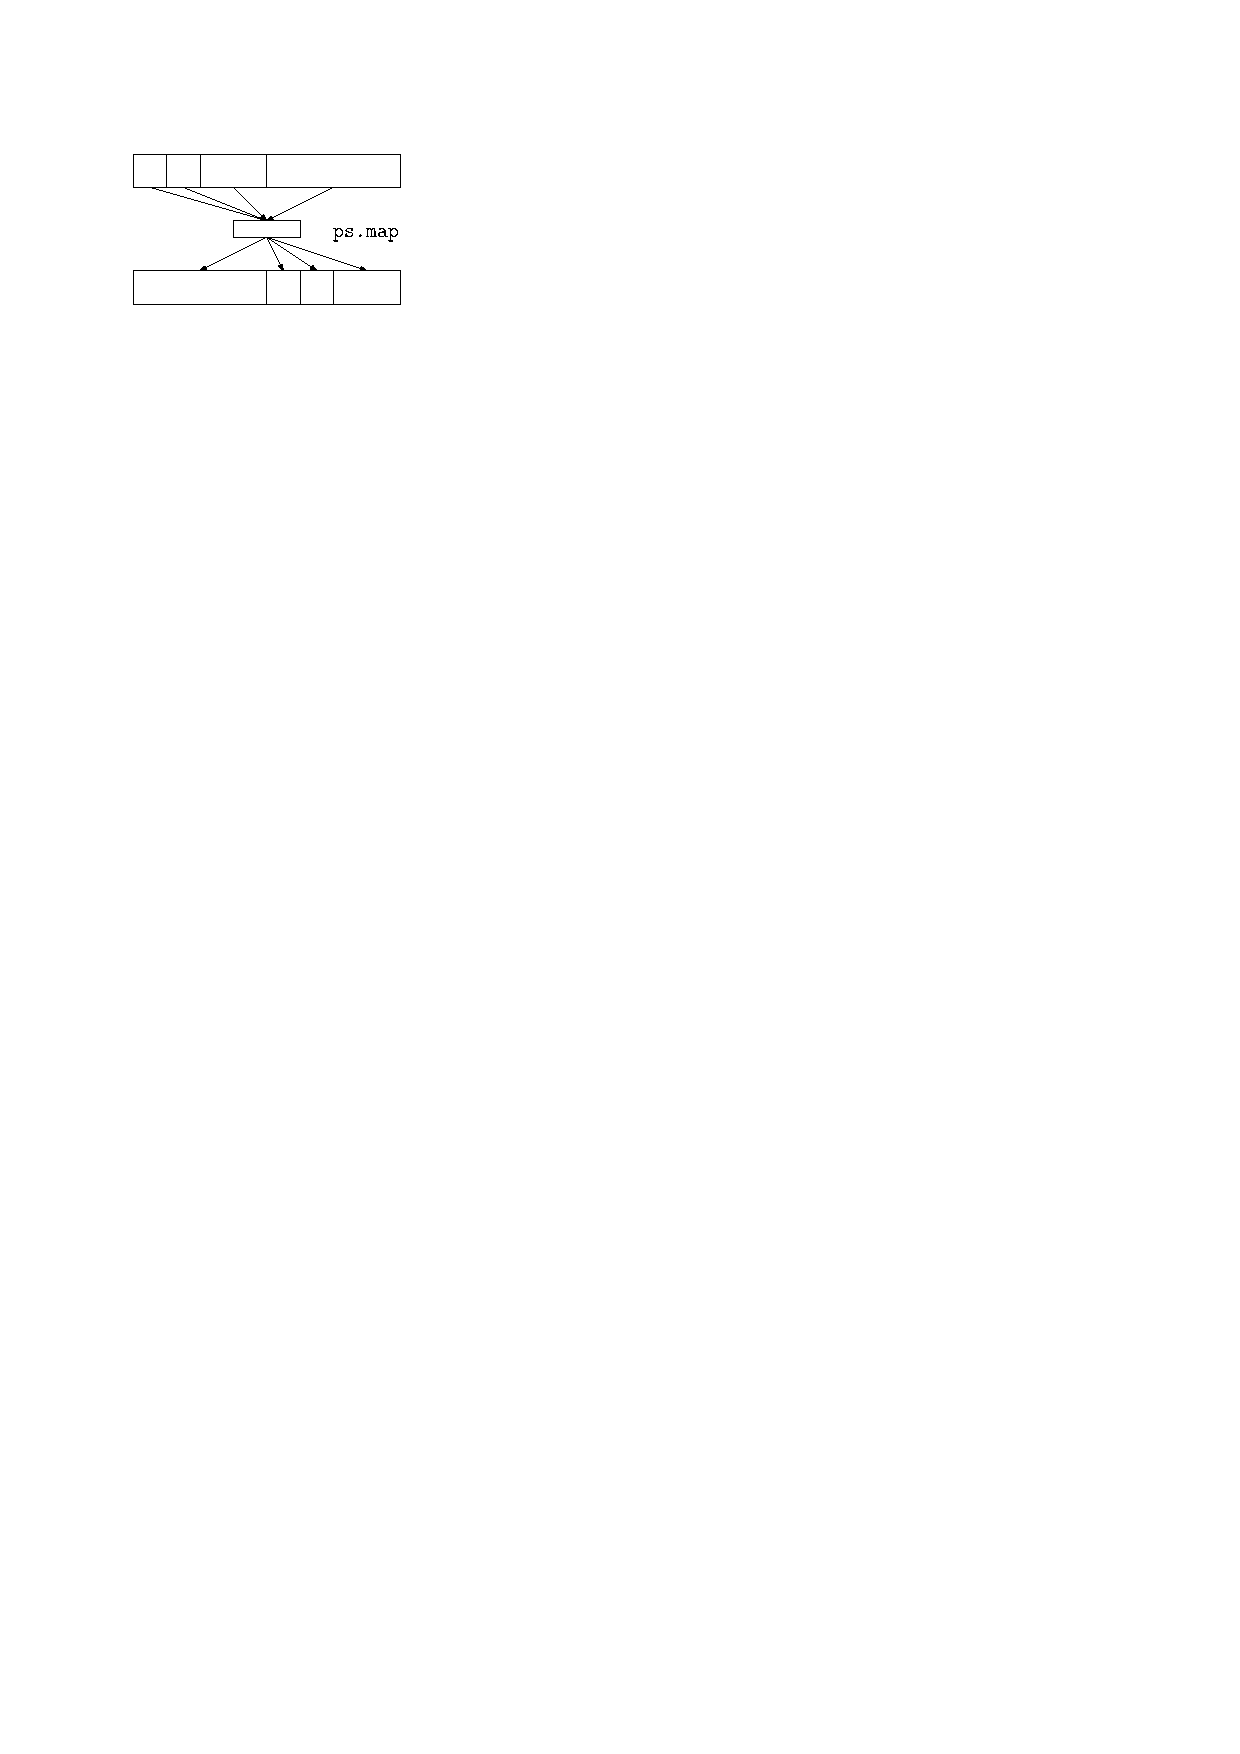
\includegraphics{barrier-free-pa}}
  \qquad
  \subfigure[\texttt{FlowArray}]{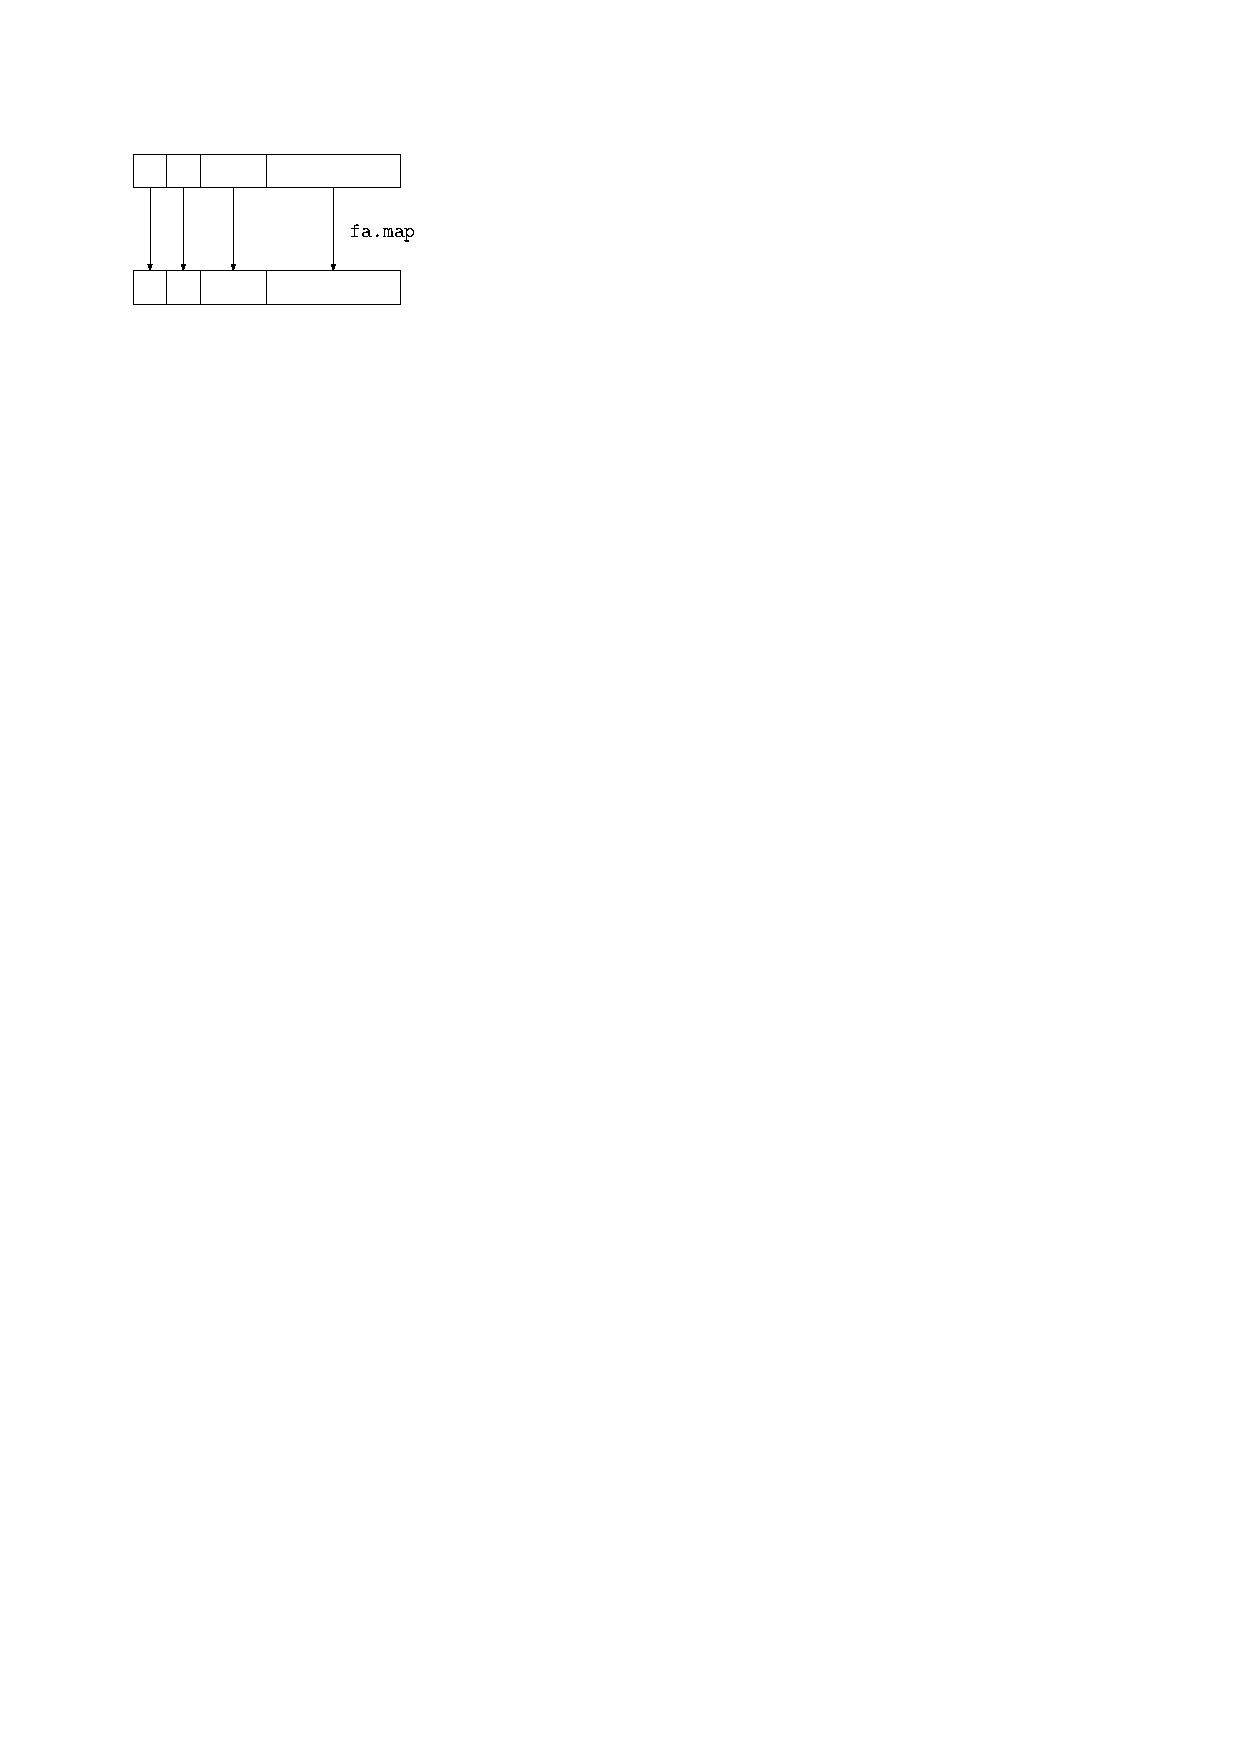
\includegraphics{barrier-free-fa}}
  \caption{Illustration of barrier-freedom of \texttt{FlowArrays}}
  \label{fig:barrier-free}
\end{figure}

\subsection{Dependency Tracking}
We'll now describe in detail what happens when a \texttt{map} is
called on a \texttt{FlowArray} depending on the different possible states of
its blocks. A block is a chunk of the \texttt{FlowArray} internal
data-array whose elements are calculated by a single worker-thread, after
the splitting (as illustrated 
in Fig.~\ref{fig:barrier-free}) has been done. It is important to
understand that dependency tracking 
happens for each block individually and hence the calculation in one
part of the \texttt{FlowArray} may advance without waiting for another
part. Fig.~\ref{fig:dep-track} illustrates the different scenarios that
may happen on a single-block level.

In the figure, the circles represent jobs: Gray circles are jobs which 
are executing or submitted to the execution queue, meaning that all 
data required to start calculation of this job is available. White
circles are in an internal queue of another job (indicated by the dashed
arrow), meaning that this calculation cannot be started yet, as some
required data is still being calculated.

The rectangles represent the data blocks of a \texttt{FlowArray} (i.e. a range
of indexes): White blocks are (partially) empty, i.e. not all elements
are calculated and a job to calculate them is still running or pending
for execution. Gray blocks are fully calculated, i.e. all elements
have their correct value and all references to calculating jobs may be
freed, since no dependency tracking has to be done for this block
anymore.

\begin{figure}
  \centering
  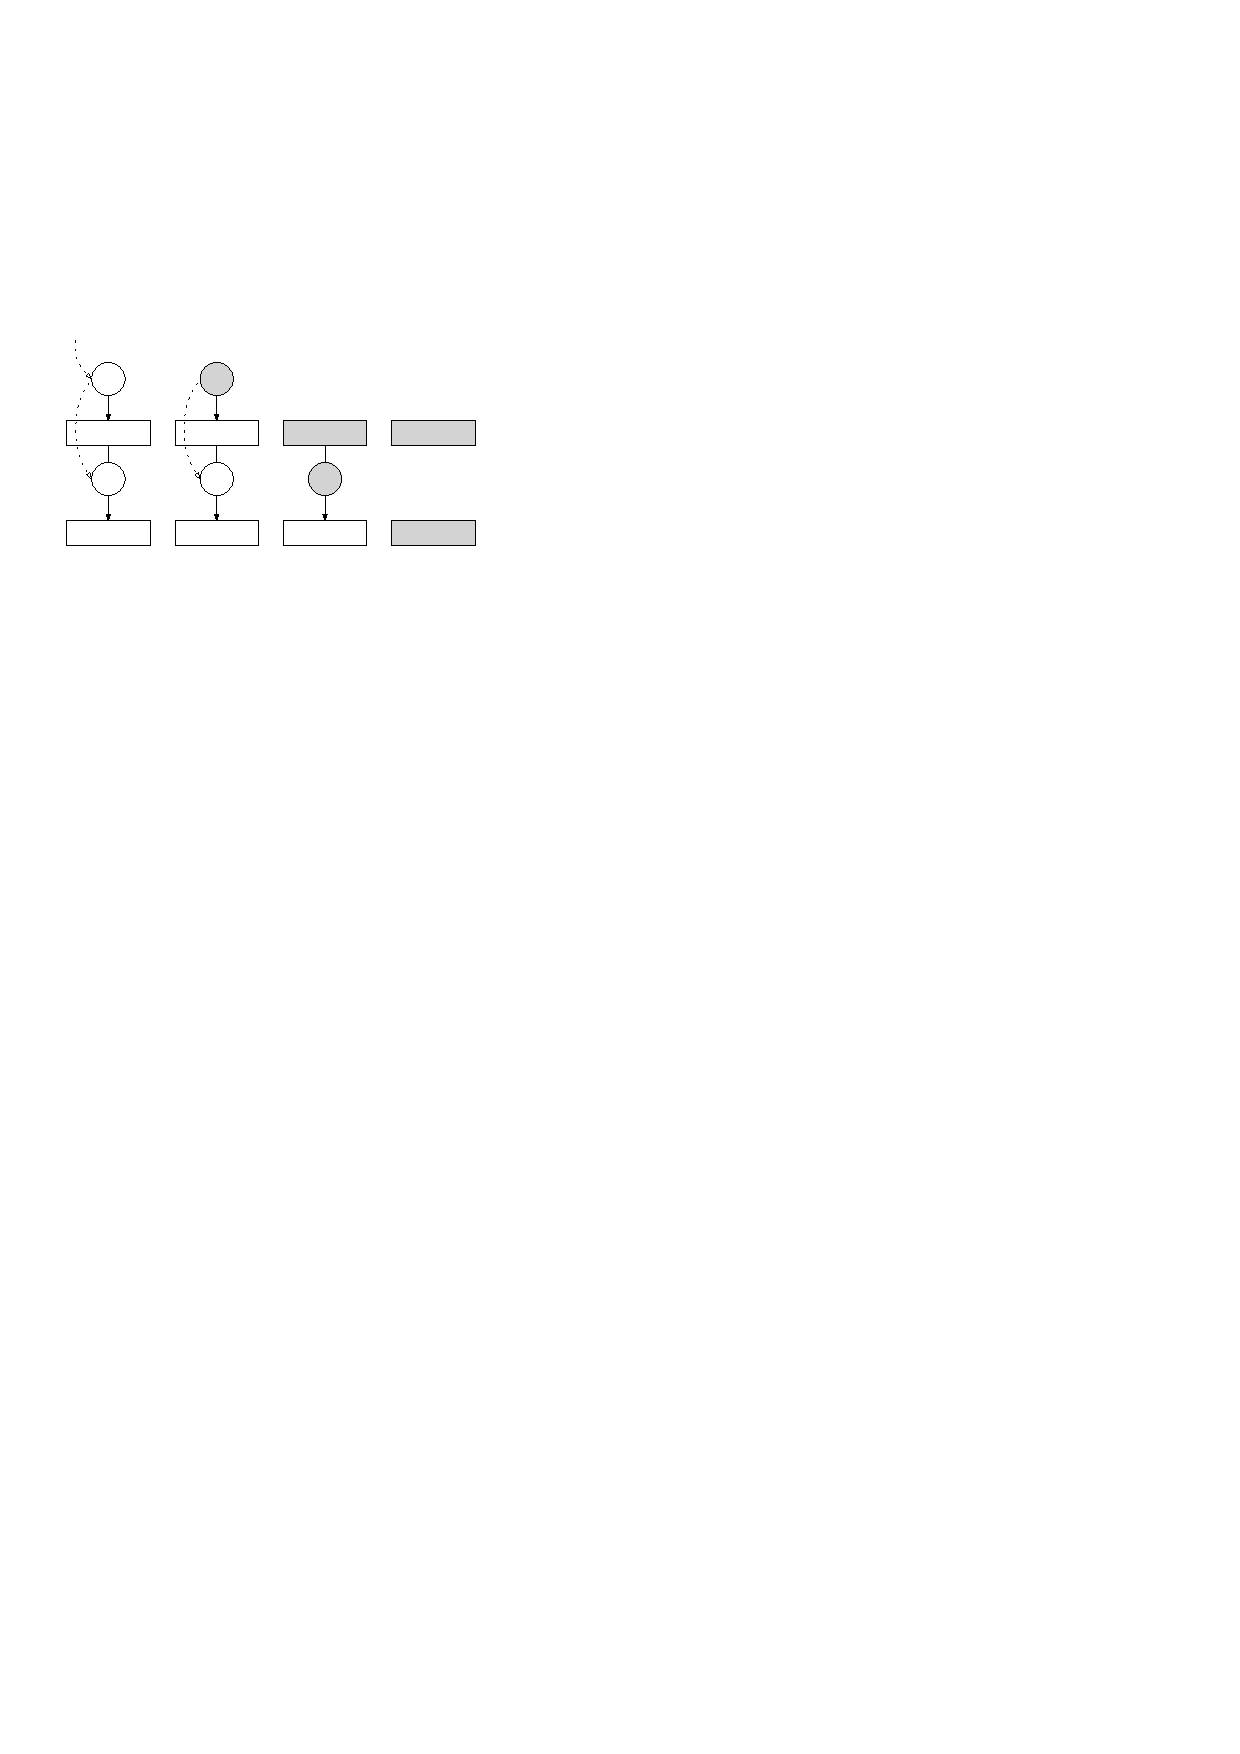
\includegraphics{dependency-tracking}
  \caption{Illustration of the dependency tracking in \texttt{FlowArrays}}
  \label{fig:dep-track}
\end{figure}

When a \texttt{map} is called on a \texttt{FlowArray}, each block chain will
start in one of the three first states (as indicated in
Fig.~\ref{fig:dep-track}) 
and then traverse each state to the right until both blocks are fully
calculated. The states are the following (from left to right):

\begin{enumerate}
\item Both blocks are not yet calculated and the job for the first
  block still depends on some other job: The second job is added to
  the first job's dependency queue.
\item The job for the first block is scheduled for execution but not
  yet finished: The second job is added to the first job's dependency
  queue.
\item Calculation of the first block is already completed: The second
  job is scheduled for execution immediately.
\item Both blocks are completely calculated.
\end{enumerate}

\subsection{Operations}
We have seen how dataflow with dependency tracking can be used in
monadic operations on the example of a \texttt{map}. In this section
we will describe the caveats of other common monadic operations on
arrays. For a complete description of what operations \texttt{FlowArrays}
support, please refer to section~\ref{ssec:flowarray}.

\subsubsection{Fold}
When doing out of order folding, each block has first to be reduced to
a single element, then these results have to be combined to the final
result. During splitting of the jobs, one can create a binary tree of
blocks along which one can later accumulate the elements;
Fig.~\ref{fig:fa-fold} illustrates this approach.

\begin{figure}
  \centering
  \subfigure[Job hierarchy]{%
    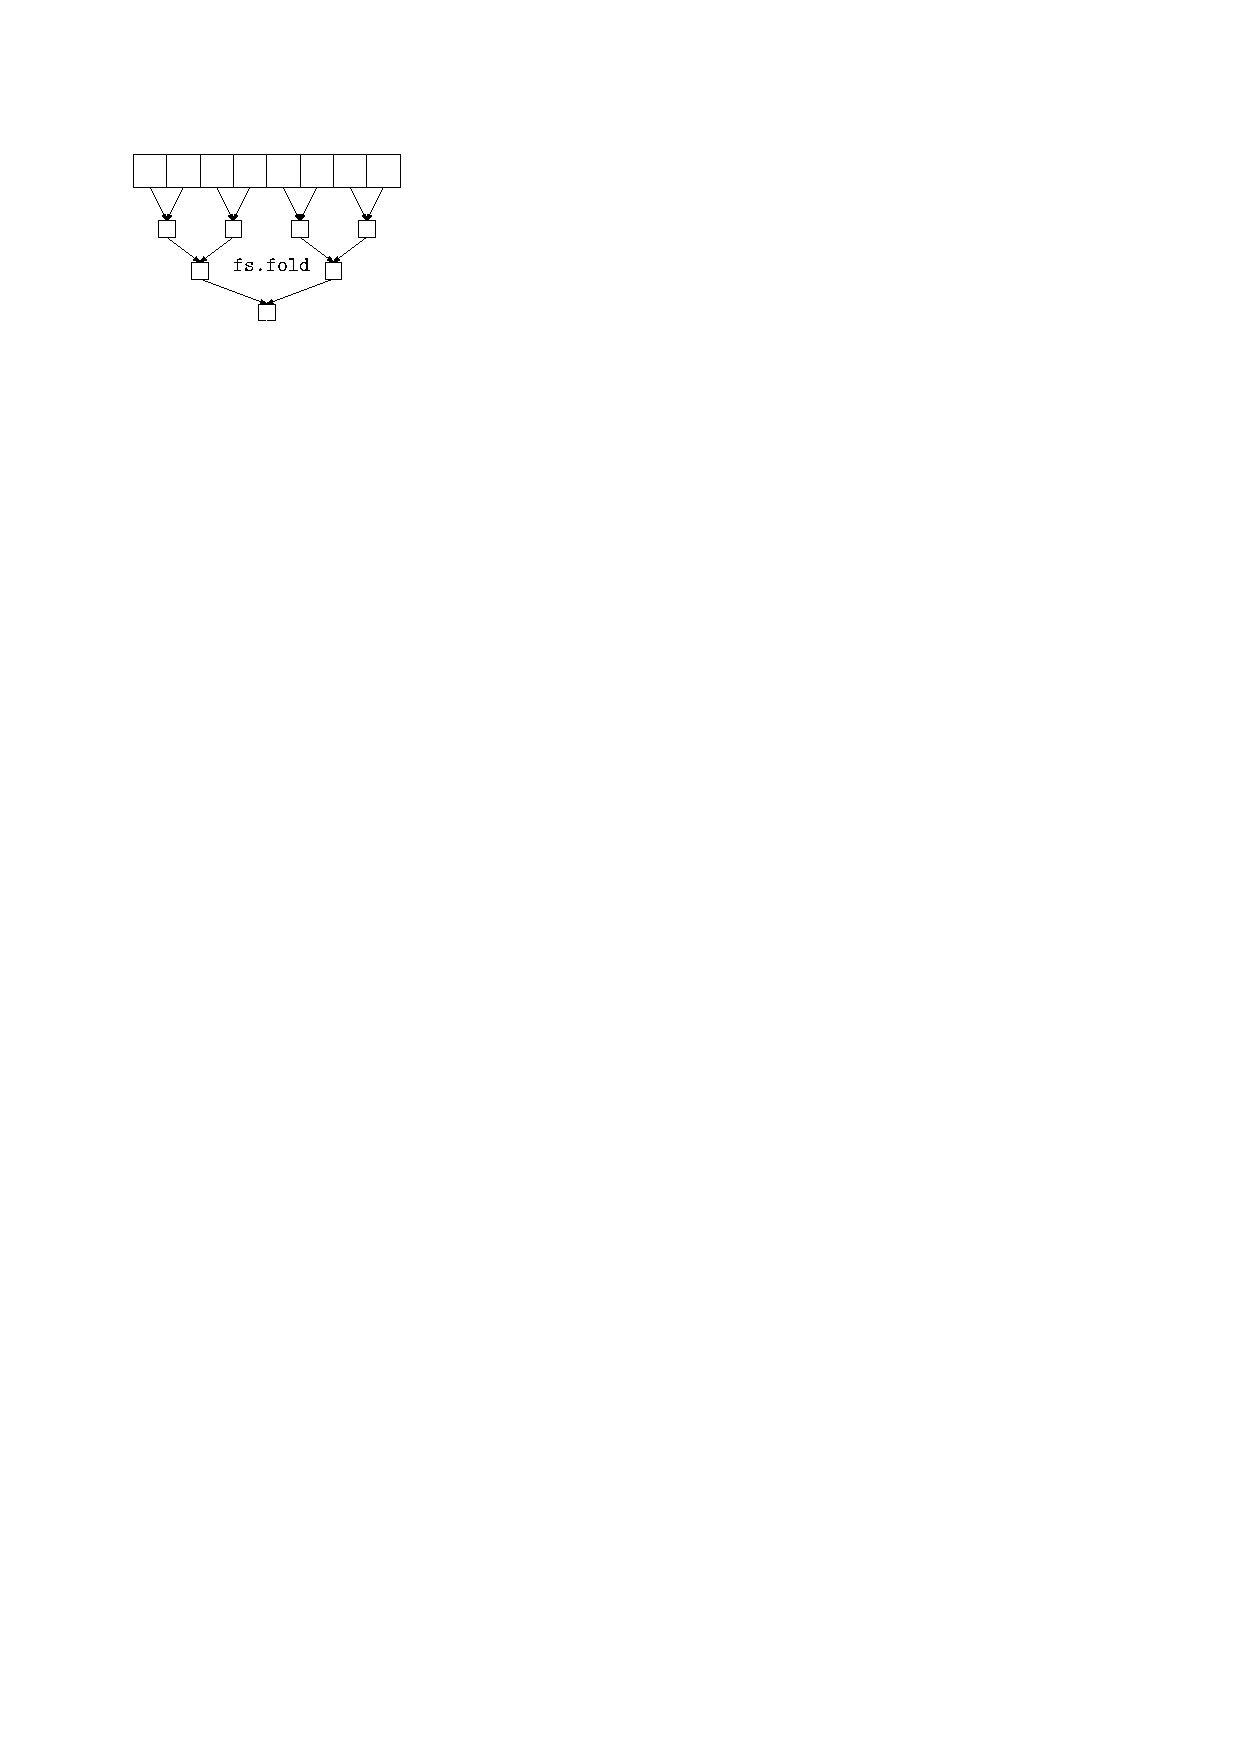
\includegraphics{fa-fold}%
    \label{fig:fa-fold}}
  \qquad
  \subfigure[Calculation]{%
    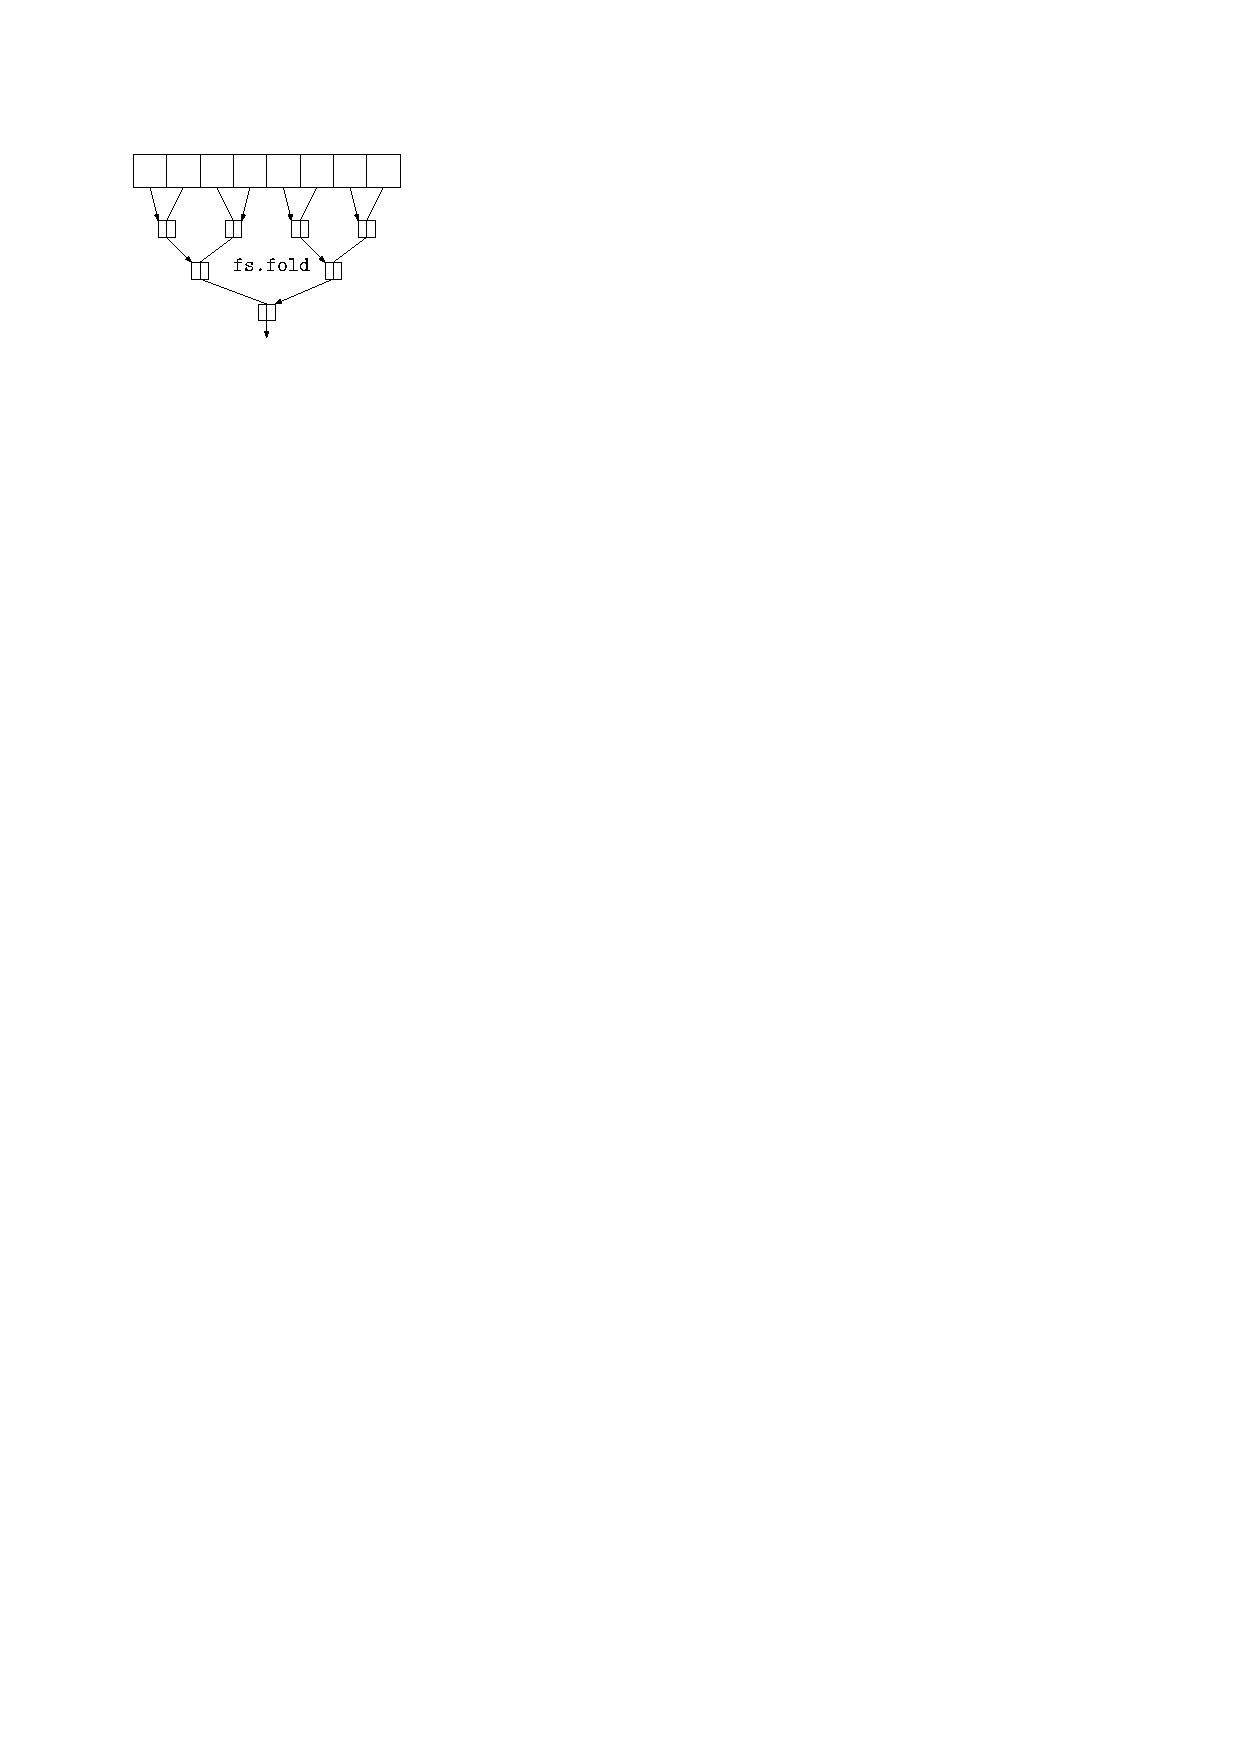
\includegraphics{fa-fold-calc}%
    \label{fig:fa-fold-calc}}
  \caption{Illustration of \texttt{fold} on a \texttt{FlowArray}}
\end{figure}

In order to keep the number of jobs (and hence the burden of managing
them) minimal, rather then spawning a single job for each accumulation
step in the tree, the job which finishes second on each node is
responsible for calculating its accumulated value (see
Fig.~\ref{fig:fa-fold-calc}). Using this scheme, the 
same number of jobs are spawned as for a \texttt{map}.

Note that this approach is preferable to a single element where
completed elements are accumulated using a CAS since the former
does preserve the order in which elements are accumulated, i.e. it
does not require the accumulation function to be commutative, only
associative.

\subsubsection{FlatMap}
\label{sssec:flatMapN}

When calling \texttt{flatMap} on a \texttt{FlowArray}, the size of the
resulting \texttt{FlowArray} is not known until the inner \texttt{FlowArrays} are
created and hence their size can be read. However, since this happens 
asynchronously, the size of the resulting \texttt{FlowArray} would not be known
at its creation. This poses several challenges:

\begin{itemize}
\item The interface of \texttt{FlowArrays} becomes more complex since the size
  of a \texttt{FlowArray} would not always be known on creation and hence the
  \texttt{size} field had to be turned into a future.
\item Increased difficulty in memory allocation: since the size of a
  \texttt{FlowArray} is not known in advance, memory allocation has to take
  place either after a barrier on the size of the \texttt{FlowArray} -- which
  we want to avoid -- or has to be done adaptively once the individual
  sizes become known which quickly turns scheduling into a
  nightmare. 
\item Increased difficulty in scheduling of subsequent calls for
  similar reasons as memory allocation.
\end{itemize}

Instead of deferring the size calculation, \texttt{FlowArrays} require
one to pass
the size of the resulting \texttt{FlowArrays} to a \texttt{flatMap}
operation 
when calling it (hence the name \texttt{flatMapN}). This greatly 
facilitates book-keeping within the \texttt{FlowArray}'s
implementation.

Further, the \texttt{FlowArray} now needs to keep track of dependencies twice:
Once, whether a sub-\texttt{FlowArray} has already been created, second,
whether a given one of its blocks is already calculated. Refer to
Fig.~\ref{fig:flatMap-dependency} for an illustration: the upper,
bigger, block holds references to the individual \texttt{FlowArrays} created by
the closure call of the \texttt{flatMapN}. The first dependency
tracking happens here: one has to check, whether the \texttt{FlowArray} for a
given index already has been created. The lower, smaller blocks are
the data blocks of the said \texttt{FlowArrays}. The second dependency tracking
happens here: being \texttt{FlowArrays}, not all their elements might already
have been calculated.

\begin{figure}
  \centering
  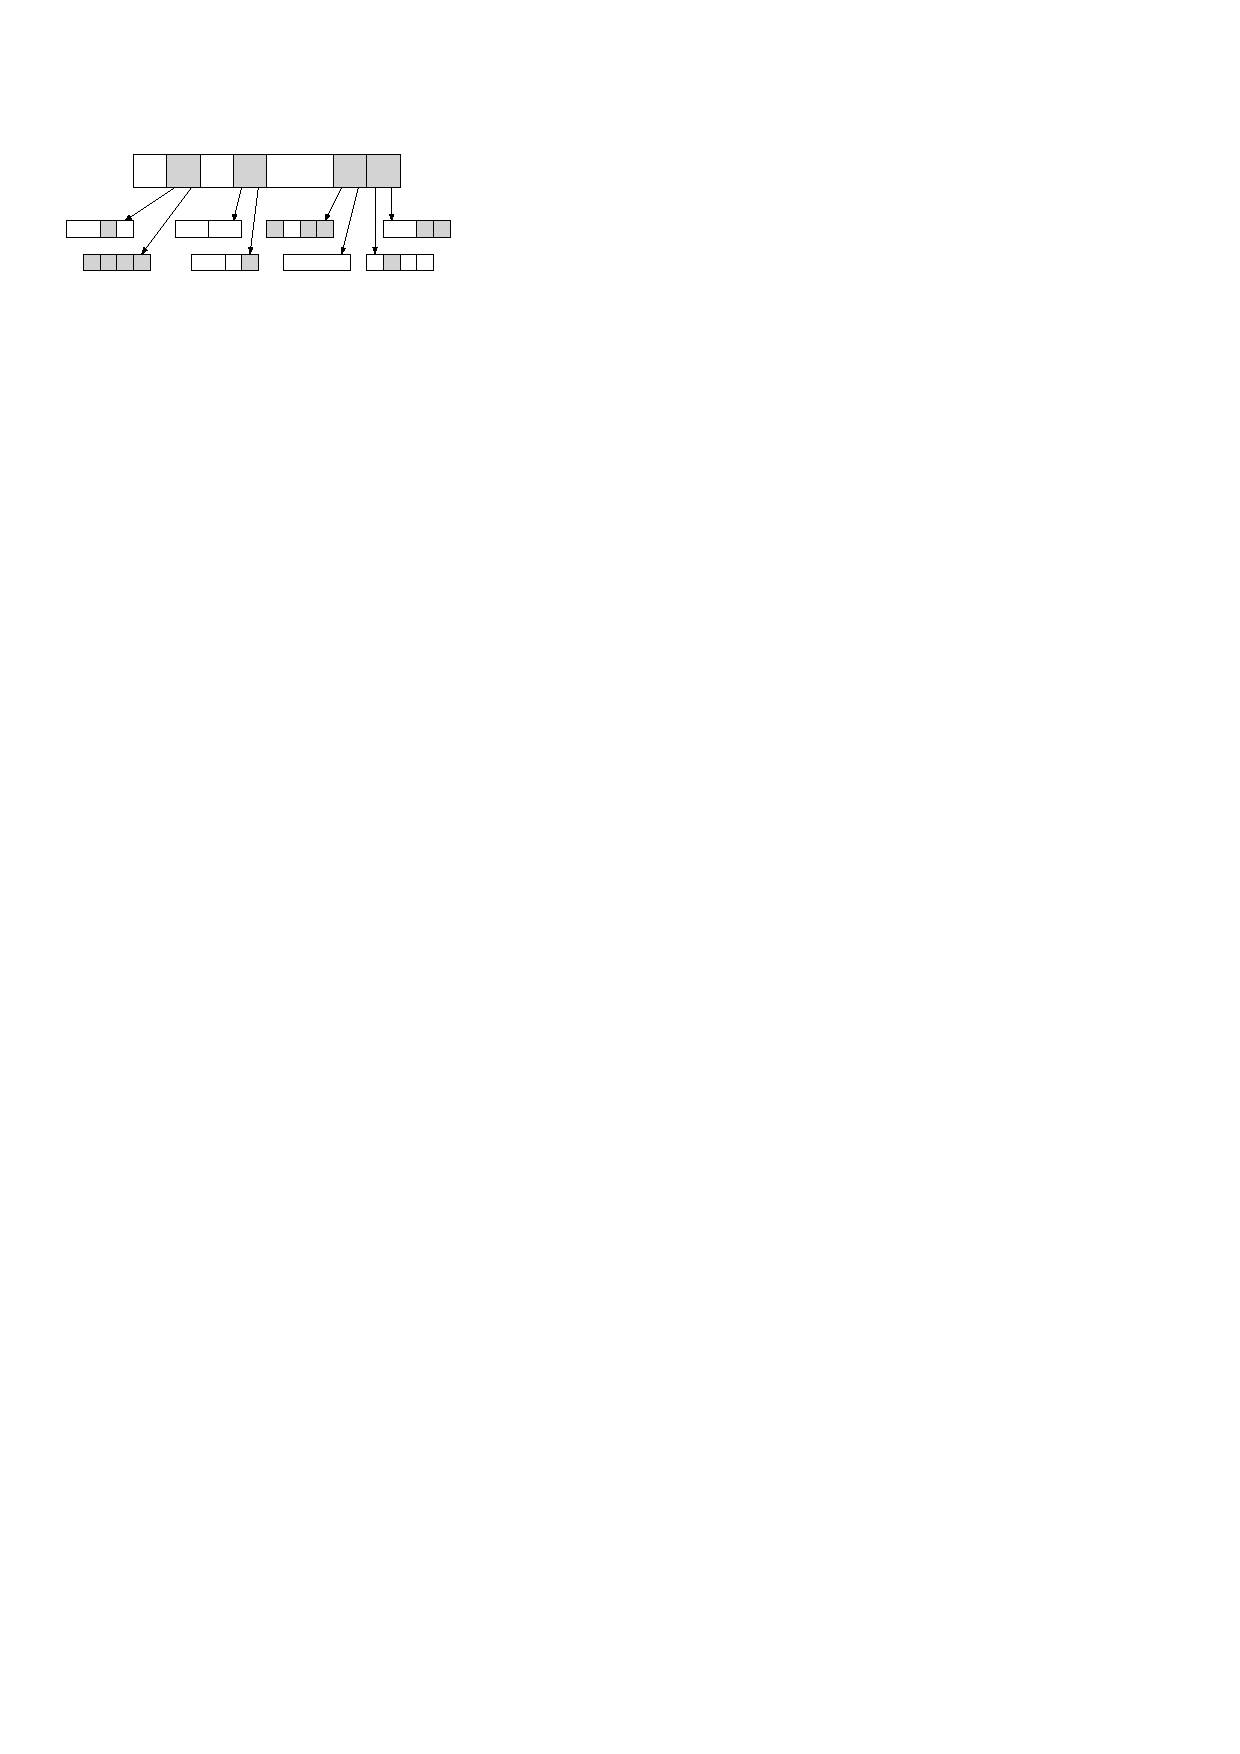
\includegraphics{flatMap-dependency}
  \caption{Illustration of dependency-tracking requirements in a
    Hierarchical \texttt{FlowArray} resulting from a \texttt{flatMap}}
  \label{fig:flatMap-dependency}
\end{figure}


In other words: to access the element with index $n$ in
such a hierarchical structure, one has to check first whether the
\texttt{FlowArray} responsible for this index is available (i.e. the \texttt{FlowArray}
with index $\lfloor \frac nN \rfloor$) and then, whether
the particular element of this \texttt{FlowArray} is already available
(i.e. element with index $n \bmod N$).

Since this tracking requires the outer \texttt{FlowArray} to keep references to
all the \texttt{FlowArrays} created by the closure call -- in order to avoid
unnecessary copying of data -- the \texttt{FlowArray} remains in this
hierarchical structure instead of being truly flattened.

When a \texttt{map} is called on one of these \emph{Hierarchical
  FlowArrays} individual \texttt{maps} are called for each sub array
and only then the resulting data is written into a flat array. This
allows to ``flatten out'' those hierarchical structures without
additional computation costs. The same is true for \texttt{folds} on
these structures.

It becomes much more interesting when we look at nested or subsequent
calls to \texttt{flatMap}: have a look at the following two
definitions.
\begin{alltt}
{\scriptsize
val fa1 = x.flatMapN(n*n)(x => x.flatMapN(n)( ... ))
val fa2 = x.flatMapN(n)(...).flatMapN(n)(...)
}
\end{alltt}
In the calculation of \texttt{fa1}, we will end up with a hierarchy of
three levels: the inner call to \texttt{flatMapN} is forced to return
a hierarchical structure as it does not a priori know what the closure
will return. But so is the outer call: it cannot flatten the hierarchical
structure from the inner call as it will only become available after
some time.

The calculation of \texttt{fa2}, will end up in a hierarchy of
two levels only: the first call to \texttt{flatMapN} will produce a 
hierarchy of two levels already. However, the second call will --
similarly to a \texttt{map} -- flatten out a level and produce another
one in return.

Note that currently throughout this scheme, the splitting happens only
in terms of the outer 
blocks, i.e. individual elements of inner \texttt{FlowArrays} are always
assigned to the same calculation blocks. This is acceptable as long as
the number of inner \texttt{FlowArrays} is relatively high.

There is currently no way to launch re-alignment of the blocks
in order to remove the arbitrary splitting imposed by the hierarchy
introduced by the \texttt{flatMapN}. While all the necessary building
blocks to do so are available and hence the implementation trivial, it
is unclear which mechanism should trigger such a
re-alignment. Exposing it to the programmer through the
\texttt{FlowArray}'s interface has him bother with issues he shouldn't
be concerned about, on the other hand finding an appropriate
heuristics might be far from easy.

For details on how the block splitting is
propagated through dependencies, please refer to
section~\ref{sec:implementation}.

\subsubsection{Zip}
When zipping, again we impose a restriction on the size: 
the two \texttt{FlowArrays} which are being zipped need to be of the same
size. This is again to ease scheduling and to keep the implementation
tractable. However, in 
this case, minor changes in the implementation could easily remove
this limitation (unlike \texttt{flatMap}, where the interface would
need to undergo a fundamental change).

Further, the splitting of the two \texttt{FlowArrays} which are being zipped
may be totally different, e.g. due to a preceding \texttt{flatMap} on
one of them. Hence re-alignment of blocks is required,
before the zipped tuples can be created. It is important to realize,
that this may inherently lead to non-symmetric scheduling behavior:
Depending on which \texttt{FlowArray} is on the ``left'' of the \texttt{zip}
call, the resulting splitting may be different, which may lead to
different speed at runtime. 

\section{Implementation}
\label{sec:implementation}

This section describes in some more detail, how the requirements
explained in section~\ref{sec:overview} are implemented. Note that
this is a simplified view and some interfaces may not be described
with all methods or all arguments of the methods. Further, methods may
be simplified (e.g. not tail-recursive for easier understanding).

\subsection{FlowArray Jobs}
The class \texttt{FAJob} is the center-piece of the whole \texttt{FlowArray}
implementation: It handles computation, task splitting and dependency
tracking. An \texttt{FAJob} has a range of array indexes it operates
on
(\texttt{start,end}) and an abstract method that does the computation
(\texttt{doCompute}). Further, the following methods are supported for
dependency tracking, splitting and scheduling:

\begin{description}
  \item[\texttt{depending(newJob: FAJob): Unit}] Submits another \texttt{FAJob} as being
    dependent on this \texttt{FAJob}. This will schedule
    \texttt{newJob}, once this \texttt{FAJob} is completed.

    For example, suppose \texttt{j1: FAJob} is responsible to
    calculate some data that \texttt{j2: FAJob} requires. One
    could write \verb|j1.depending(j2)| which will execute a given
    junk of \texttt{j2} only, once the corresponding junk of
    \texttt{j1} is completed.
  \item[\texttt{split(): Unit}] Splits this job into two
    sub jobs. It forces dependent tasks to be split as well, and hands off
    dependencies (see next section for details on splitting). This
    method is called when computation of a \texttt{FAJob} starts and
    its size is above the threshold for exponential splitting.
  \item[\texttt{done: Boolean}] Checks whether this \texttt{FAJob} is
    done. It queries sub jobs if this \texttt{FAJob} is split.

    This method is used for example in the final aggregation of a 
    \texttt{fold} (see Fig.~\ref{fig:fa-fold-calc} on
    page~\pageref{fig:fa-fold-calc}) to check if the other job is
    already completed. Please refer to Fig.~\ref{fig:fa-fold-code} for
    pseudo code of this aggregation: the method \texttt{jobDone} is
    called each time a sub job is completed. It checks if both jobs
    are completed, fetches both results and combines them.

\begin{figure}    
\begin{alltt}
{\scriptsize
def jobDone() \{
  val (sj1, sj2) = subTasks
  if (sj1.done && sj2.done) \{
    this.result = combine(sj1.result, sj2.result)
  \}
  
  // Do other stuff (notification, finalization)
\}
}
\end{alltt}
\caption{Aggregation of results of different jobs during a
  \texttt{fold}}
\label{fig:fa-fold-code}
\end{figure}

  \item[\texttt{sliceJobs(from: Int, to: Int): Option[(Seq[FAJob],
      Boolean)]}] Returns the jobs which are responsible for
    calculating a given slice. In some cases, all the jobs responsible 
    for the slice might not be known yet (for example when doing
    double-dependency tracking after a \texttt{flatMapN}, see
    section~\ref{sssec:flatMapN}). In this case, the Boolean flag
    indicates that the caller has to call this method again, once all
    the jobs returned from the current call are completed. If the
    calculation of the queried slice is completed, the method returns
    \texttt{None}.

    This method is for example used to re-align the splitting
    patterns when two \texttt{FlowArrays} are zipped or when
    operating on slices of a \texttt{FlowArray} (through
    \texttt{FlowArraySliceViews}, see section~\ref{sssec:slice-views}
    on page~\pageref{sssec:slice-views}).
  \item[\texttt{delegateThen(d: Seq[FAJob])(thn: () => Unit): Unit}]
    This method may be called from inside the \texttt{doCompute}
    method only. It halts calculation of this \texttt{FAJob}, until
    all jobs in \texttt{d} are completed. It then (optionally)
    executes the closure \texttt{thn}. This is implemented using an
    observer pattern on the \texttt{FAJobs} in \texttt{d}.

    Delegation is often used in conjunction with \texttt{sliceJobs}
    when re-aligning splittings, for example when calling \texttt{x
      zip y}; the internal scheduling of \texttt{FAJobs} ensures 
    that for a given chunk the corresponding values in \texttt{x} are
    calculated. The \texttt{zipJob} then queries the job responsible
    for calculating the elements in this chunk in \texttt{y} and
    delegates to it. Finally -- using the \texttt{thn} closure -- it
    actually creates the zipped tuple and stores it in the destination 
    \texttt{FlowArray}.
\end{description}

\subsubsection{State Machine}
You can find the state machine of an \texttt{FAJob} in
Fig.~\ref{fig:fajob-state}. We give a description of each state: 

\begin{description}
\item[Pend] Initial state. Execution of this \texttt{FAJob} is
  \emph{pending}, no dependencies have been recorded.
\item[PNext] Execution of this \texttt{FAJob} is
  \emph{pending}, the \emph{next}, depending \texttt{FAJob} has been
  submitted.
\item[Split] This \texttt{FAJob} is \emph{split}. Execution is
  delegated to two smaller sub jobs. This \texttt{FAJob} aggregates
  their completion state.
\item[Spl'ing] This \texttt{FAJob} is being split. Splitting of this
  job is completed, \emph{splitting} of depending jobs is still
  pending.
\item[Calc] This \texttt{FAJob} is being \emph{calculated}. This state
  is internally represented with either \textbf{Pend} or
  \textbf{PNext}. A job that started execution cannot be split
  anymore.
\item[Deleg] This \texttt{FAJob} has started calculation but is
  currently \emph{delegated} other \texttt{FAJobs} and is waiting for
  their completion.
\item[Done] Calculation of this \texttt{FAJob} is
  \emph{done}. Possible depending jobs are scheduled for execution
  once this state is reached.
\end{description}

\begin{figure}
  \centering
  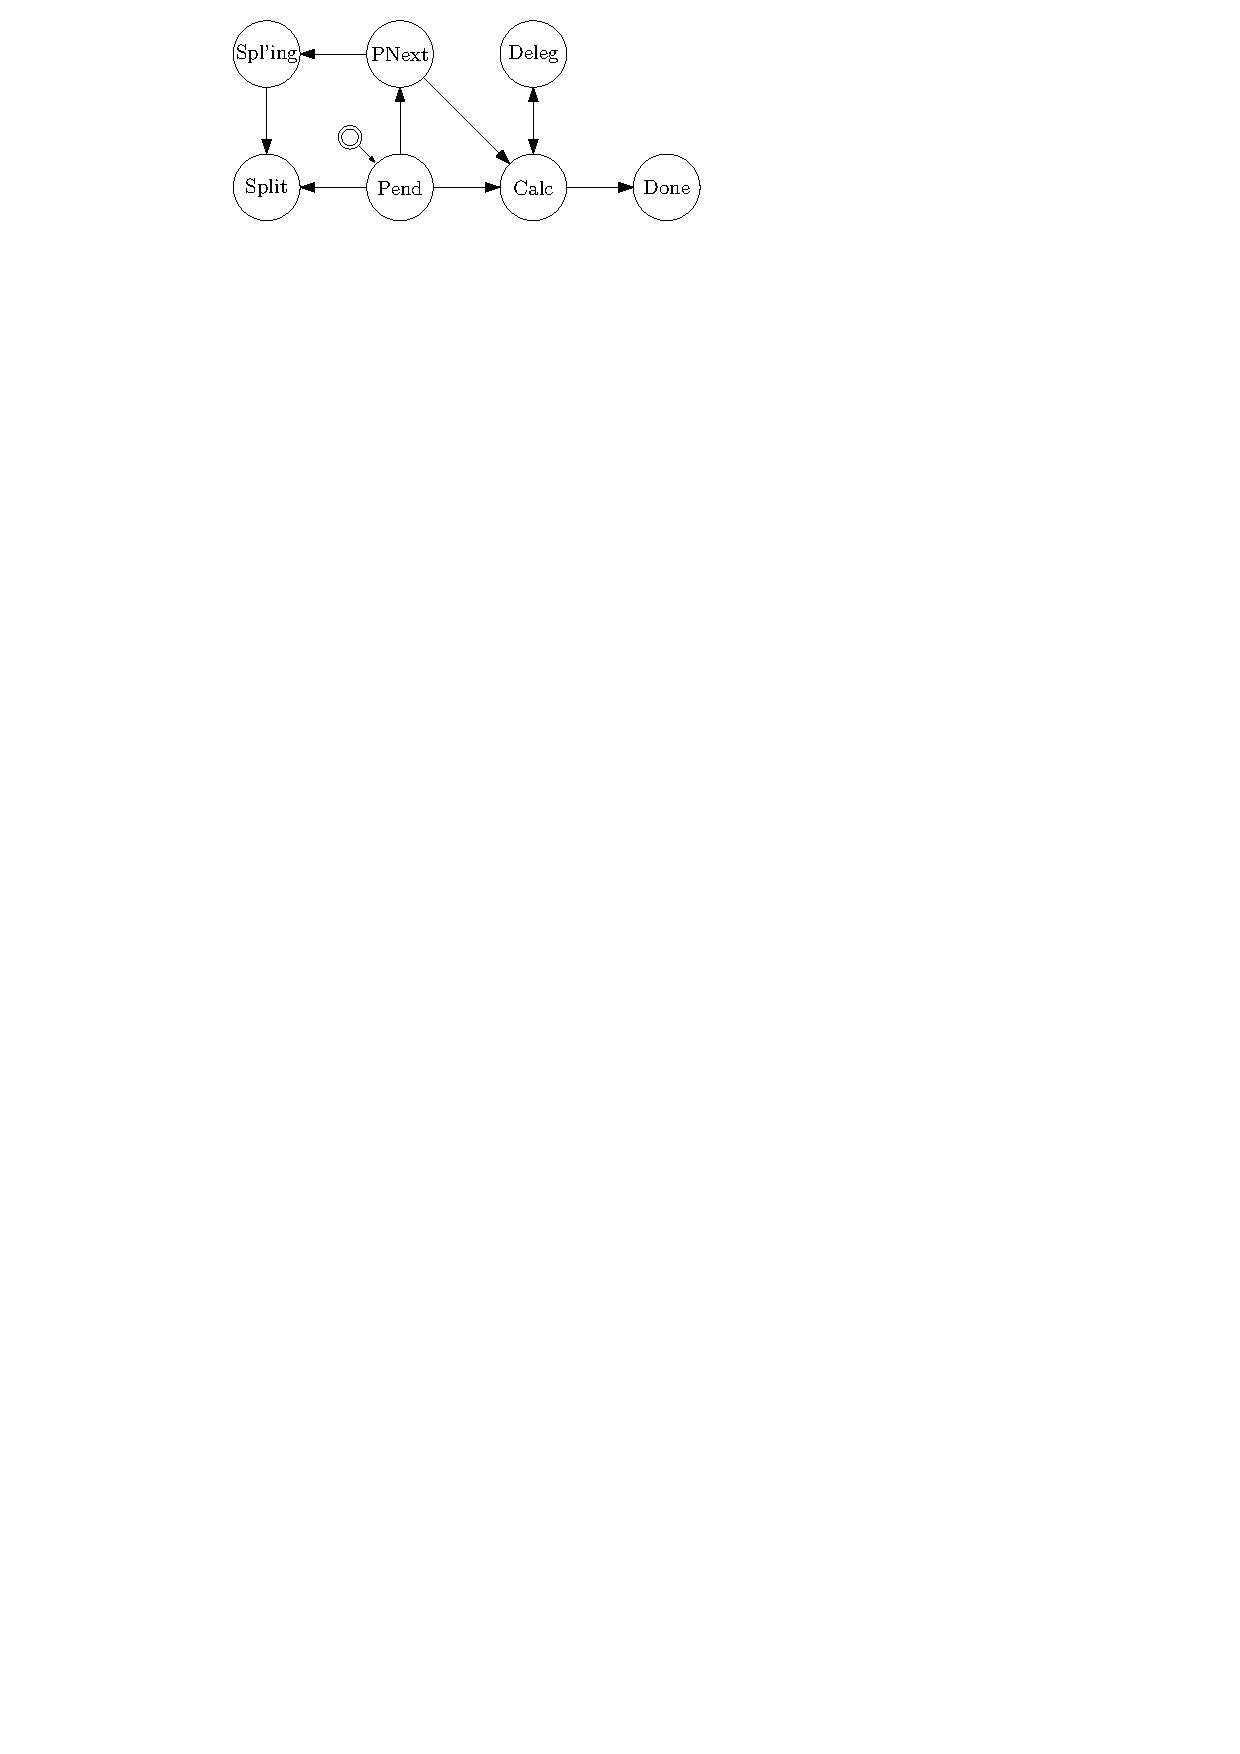
\includegraphics{fajob-state}
  \caption{State machine of \texttt{FAJob}}
  \label{fig:fajob-state}
\end{figure}

\subsubsection{Splitting}
When calling \texttt{split} on a \texttt{FAJob}, two things have to be
done:
\begin{enumerate}
\item Split the job in two smaller sub jobs of (more or less) equal
  size.
\item Split the dependent jobs and delegate the dependency to the
  sub jobs: we would like to have dependency tracking on individual
  block level, i.e. on the splitting level on which the calculation is 
  done. This is crucial in order to allow for dependent jobs to start
  off as soon as possible (otherwise we have a barrier and are back in
  the ages of \texttt{ParArrays}).
\end{enumerate}

Point one is easy: divide the range of the \texttt{FAJob} into two
(more or less) equal ranges and create two new \texttt{FAJobs} with
those ranges.

Point two is a bit more tricky. Please refer to
Fig.~\ref{fig:split-ill}
for an illustration of how this is done. You can find pseudo code in
Fig.~\ref{fig:split-code}. The idea is the following: First, create the
two sub jobs and set the state of this \texttt{FAJob} to
\texttt{Splitting}. It is now ``locked'' for any other operation,
i.e. any
other operation must help the splitting first (as the implementation
is lock-free). Next, the dependent job must be split
(recursively). Once this is done, the dependants of the sub jobs may be
set to these newly created sub jobs. Finally the state of this
\texttt{FAJob} may be set to \texttt{Split}.

\begin{figure}
  \centering
  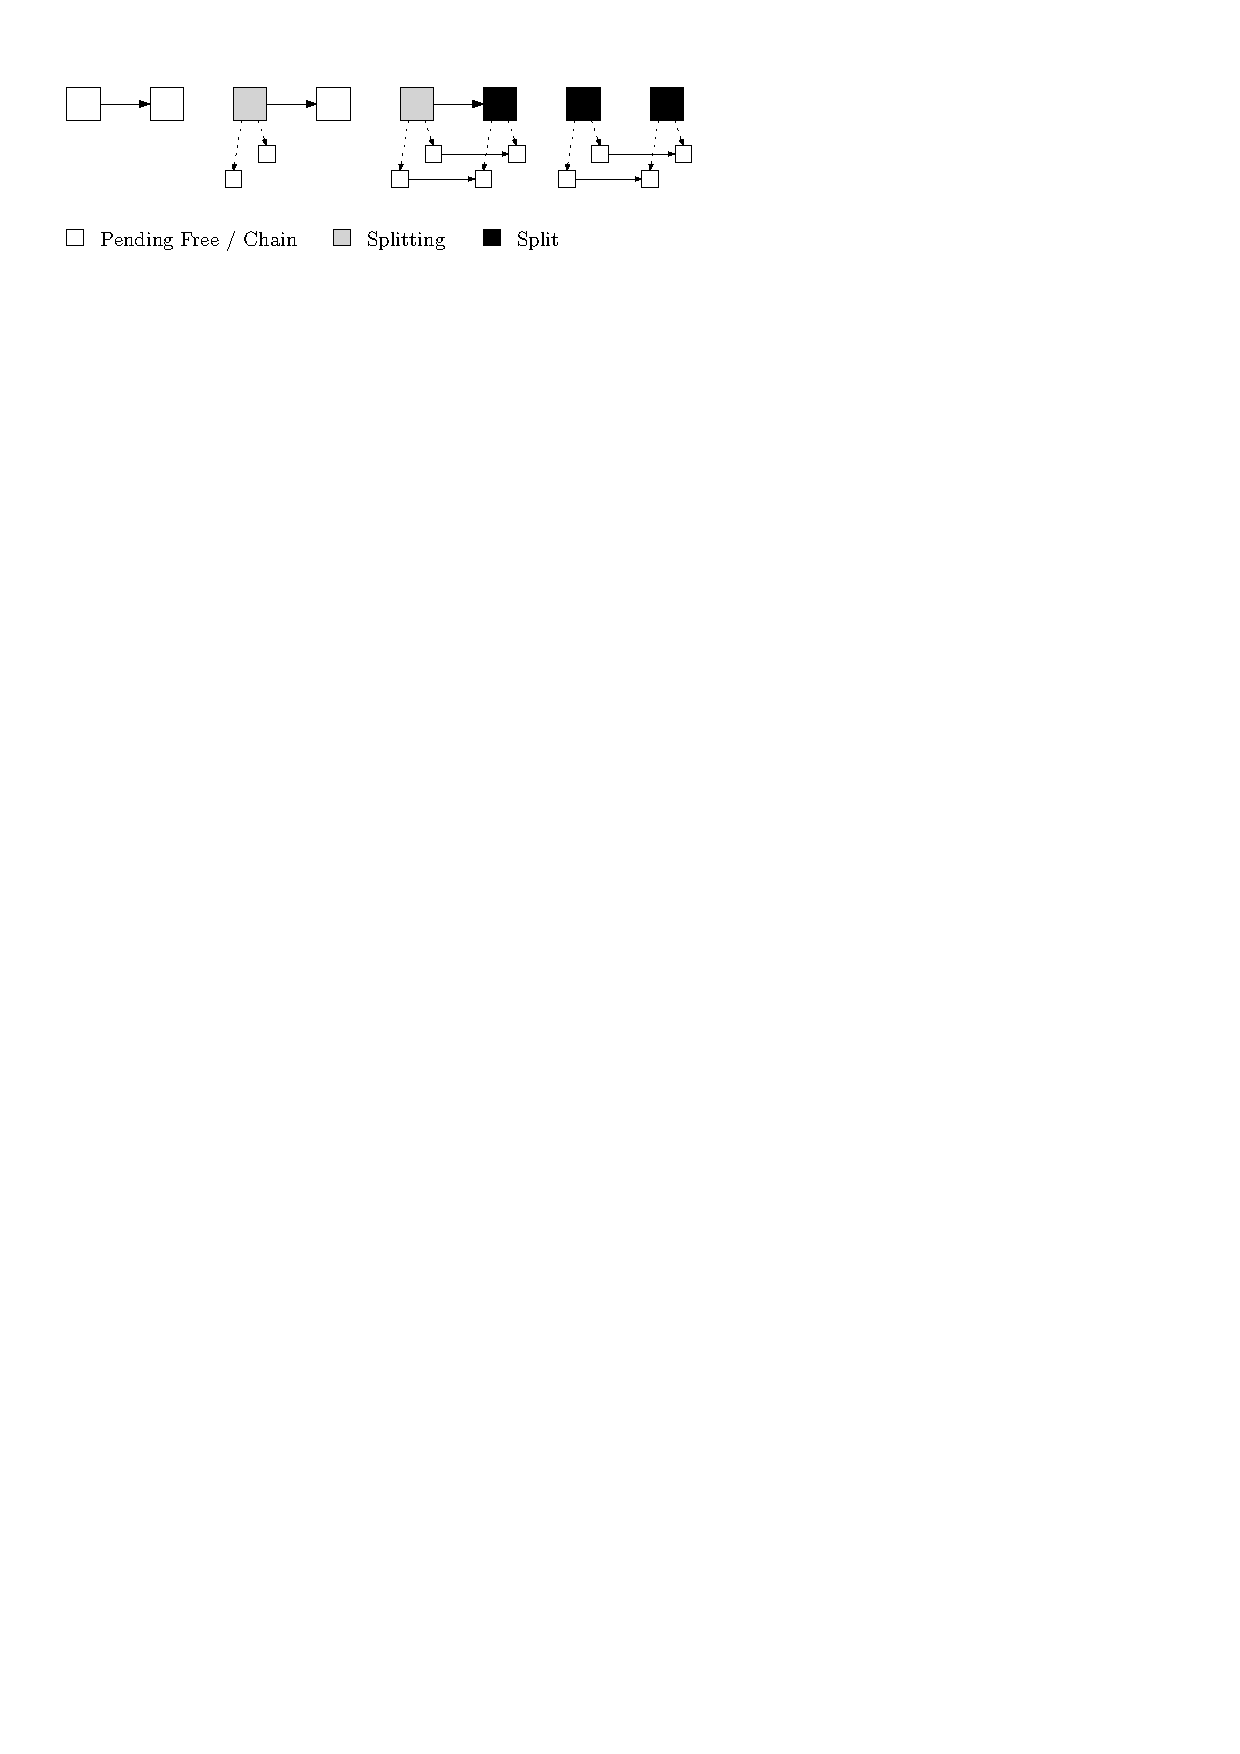
\includegraphics[trim = 0mm 18mm 0mm 0mm, clip]{split}
  \caption{Step-by-step illustration of splitting with dependencies}
  \label{fig:split-ill}
\end{figure}

\begin{figure}
\begin{minipage}[t]{7cm}
\begin{alltt}
{\scriptsize
def split(): (FAJob, FAJob) = state match \{
  case os@PendingFree =>
    val sj = newSubJobs
    if (CAS(state, os, Split(sj))) sj
    else split()
  case os@PendingChain(nextJob) =>
    val sj = newSubJobs
    CAS(state, os, Splitting(sj, nextJob))
    split()
  case os@Splitting(j1, j2, nextJob) =>
    val (nj1, nj2) = nextJob.split()
    j1.setNext(nj1); j2.setNext(nj2)
    CAS(state, os, Split(j1, j2))
    (j1, j2)
  case Split(j1, j2) => (j1, j2)
  case _ => error("Job already started")
\}
}
\end{alltt}
\end{minipage}
\begin{minipage}[t]{4cm}
\begin{alltt}
{\scriptsize
def compute() \{
  if (needSplit) \{
    val (j1, j2) = split()
    invokeAll(j1, j2)
  \} else \{
    doCompute()
  \}
\}
}
\end{alltt}
\end{minipage}
\caption{Pseudo-code for splitting and how splitting is invoked upon
  computation}
\label{fig:split-code}
\end{figure}

\subsection{FlowArray}
\label{ssec:flowarray}
\texttt{FlowArrays} are the trait exposed to the API user. They (currently)
support the following common monadic operations \texttt{map},
\texttt{fold}, \texttt{flatMapN}\footnote{See
  section~\ref{sssec:flatMapN} on why the \texttt{N} in
  \texttt{flatMapN}}, \texttt{zip}, \texttt{slice}, \texttt{flatten}
and the generator \texttt{tabulate}.

Additionally, the slightly strange operation \texttt{transpose} is
supported
to allow for matrix multiplication. For a more detailed view on 
certain operations, have a look at
section~\ref{ssec:imp-operations}. Throughout the following sections,
the operation \texttt{map} is used as an example.

Internally, two major types exist: \emph{Concrete FlowArrays} and
\emph{Views}. Concrete \texttt{FlowArrays} store actual data -- the most
trivial being the \texttt{FlatFlowArray}, which just wraps around an
array. Views on the other hand expose data from
concrete \texttt{FlowArrays} under a different form -- currently the
only supported view is the \texttt{FlowArraySliceView} which exposes
only a slice of another \texttt{FlowArray}. These internal types will be
described later on.

\subsubsection{Job Dispatch}
Job creation for monadic operations is handled through the abstract
method \texttt{dispatch}, which allows to dispatch a job specified by
a closure -- a \texttt{JobGen} -- to operate on a given range of the
\texttt{FlowArray} and returns the job which handles the block dependency
management for this calculation. Rather then specifying the exact job
to be executed when dispatching, a way of creating jobs has to be 
specified since in some cases multiple such jobs have to be created
(see the part about \texttt{HierarchicalFlowArrays} in this
section). Fig.~\ref{fig:dispatch-code} shows the 
signatures for \texttt{dispatch} and
\texttt{JobGen}. Fig.~\ref{fig:dispatch-example} shows how dispatch
can be used to implement the monadic operation \texttt{map}.

\begin{figure}
\begin{minipage}[t]{6cm}
\begin{alltt}
{\scriptsize
def dispatch(
  gen: JobGen[A],
  dstOffset: Int = 0,
  srcOffset: Int = 0,
  length: Int = this.size
): FAJob
// operates on whole FlowArray when
// called with default arguments
}
\end{alltt}
\end{minipage}
\begin{minipage}[t]{7cm}
\begin{alltt}
{\scriptsize
trait JobGen[A] \{
  def apply(
    src: FlatFlowArray[A],
    dstOffset: Int,
    srcOffset: Int,
    length: Int
  ): FAJob
\}
}
\end{alltt}
\end{minipage}
\caption{Signatures for \texttt{dispatch} and \texttt{JobGen}, }
\label{fig:dispatch-code}
\end{figure}

\begin{figure}
\begin{alltt}
{\scriptsize
def map[B](f: A => B): FlowArray[B] = \{
    val ret = newFlowArray[B](this.size)
    val job = this.dispatch(FAMapJob(ret, f))
    ret.generatedBy(job)
    ret
\}

// Comments:
//  FAMapJob(ret: FlowArray[B], f: A => B)
//    returns a JobGen[A] that creates FAJobs writing to ret using f
//  FlowArray.generatedBy(j: FAJob): Unit
//    sets j as generating job on the given FlowArray
}
\end{alltt}
\caption{Example usage of \texttt{dispatch} in the implementation of
  \texttt{map}.}
\label{fig:dispatch-example}
\end{figure}

When dispatching, it is important to note that the target of the
operation, which may be another \texttt{FlowArray} as in the case of
\texttt{map}, or a future in case of a \texttt{fold} -- is only
referenced by the \texttt{JobGen}: In the \texttt{map} example, the
statement \texttt{FAMapJob(ret, f)} creates a
\texttt{JobGen} which writes to \texttt{ret} using a transformation
function \texttt{f}. We therefore see, that the dispatching \texttt{FlowArray}
does not know the target of the operation (and does not need to
know). This allows us to use the same dispatch construct for more
complex operations (such as \texttt{flatMap}).

\subsubsection{Blocking}
\texttt{FlowArrays} also support blocking to actually retrieve the data that
has been (or will be) calculated. The operation \texttt{blocking} on
the \texttt{FlowArray} suspends execution of the calling thread until all
calculation is done and then returns the data as array. This may
require copying or consolidation of data (for example when
\texttt{blocking} is called on a view).

\subsubsection{FlatFlowArray}
The simplest case of a concrete implementation of a \texttt{FlowArray}: Just a
wrapper around a simple array which handles the completion and the
dependency tracking. The \texttt{dispatch} method calls the
\texttt{JobGen} directly (as its signature suggests), the
\texttt{blocking} method waits for the assigned job to complete and
then just returns a reference to the internal array.

\subsubsection{Slice Views}
\label{sssec:slice-views}
\texttt{FlowArraySliceViews} wrap around a \texttt{ConcreteFlowArray}
(i.e. a \texttt{FlatFlowArray} or a \texttt{HierFlowArray})
and expose a given part of it. The \texttt{dispatch} method adjusts 
offset and length and proxies the call to the \texttt{dispatch} method
of the inner
\texttt{ConcreteFlowArray}. The \texttt{blocking} method waits for the
smallest covering sub job of the inner \texttt{ConcreteFlowArray} and
then copies the required elements to a new array. Note that this
behavior might cause a calling thread to block for longer than
actually required.

\texttt{FlowArraySliceViews} are used when \texttt{slice} is called on
a \texttt{FlowArray}, which is useful for matrix multiplication.

\subsubsection{Hierarchical FlowArrays}
\texttt{HierFlowArrays} are the result of \texttt{flatMapN} operations
(see section~\ref{sssec:flatMapN} for the big picture). This is by far
the most complex concrete implementation of a \texttt{FlowArray}. The
\texttt{dispatch} method needs to dispatch a job for each inner
\texttt{FlowArray} of the \texttt{HierFlowArrays}. However, since the number of
inner \texttt{FlowArrays} is big (otherwise something different than a \texttt{FlowArray}
should have been used), 
this needs to be done asynchronously. Further, the multiple dispatched
jobs need then to be waited on and regrouped by the outer job in order
to fulfill the whole dependency tracking requirement (remember
Fig.~\ref{fig:flatMap-dependency} on
page~\ref{fig:flatMap-dependency} for an illustration on the
double dependency tracking that is required). All this is handled by a 
special job, the \texttt{FADispatchJob}.

The \texttt{blocking} method needs to flatten the hierarchical
structure into a single array by copying the data from the inner
\texttt{FlowArrays}. This copying is somewhat unnecessary -- which 
was the reason for the creation of Hierarchical \texttt{FlowArrays} in the
first place; currently, \texttt{flatMapped} data has to be copied only when
retrieving results, not in a calculation flow. Nevertheless, one might
further improve on this by providing indexed access to elements only
in \texttt{FlowArrays} instead of requiring to return a reference to a full
array.

\subsection{Operations}
\label{ssec:imp-operations}
This section describes some operations on \texttt{FlowArrays} which do not fit
entirely into the \texttt{FAJob} framework or require some extensions
to it.

\subsubsection{Flatten}
For the same reasons as \texttt{flatMapN} requires the size of the
inner arrays, the \texttt{flatten} operation on \texttt{FlowArrays} requires
the size of the inner \texttt{FlowArray} to be given (and all inner \texttt{FlowArrays}
to have the same size for that matter). Thanks to hierarchical
\texttt{FlowArrays}, the implementation of \texttt{flatten} is easy:

\begin{description}
\item[\texttt{FlatFlowArrays}] are simply converted into hierarchical
  \texttt{FlowArrays} with the same data array (and the inner size given in the
  argument).
\item[\texttt{FlowArraySliceViews}] currently flatten the underlying
  concrete array and return a new view on it. This behavior should and
  can easily be improved in the future.
\item[\texttt{HierFlowArrays}] push the flatten call down to their
  inner arrays (which might in turn push it down to their inner
  arrays), until they reach a \texttt{FlatFlowArray}, which will then
  be converted into a \texttt{HierFlowArray}.
\end{description}

To retain evidences about the types inside the current \texttt{FlowArray} when
flatting, implicit arguments are used together with the
\texttt{CanFlatten} type (defined in the package object).

\subsubsection{Transpose}
This operation has specifically been written to implement matrix
multiplication with \texttt{FlowArrays}. It interprets the array as a
two-dimensional array given a step size (i.e. one dimension of the
array) and transposes it. The indexes are therefore altered as
follows (see Fig.~\ref{fig:transpose} for an illustration):
\[ i_n = \lfloor i_o / d_1 \rfloor + (i_o \bmod d_1) * d_2 \qquad (d_1
\cdot d_2 = n)\]
where $i_o,\ i_n$ are the old and new indexes, $d_1,\ d_2$ are the two
dimensions, $n$ the size of the \texttt{FlowArray}. This is currently the only
operation that changes the order of the elements in a \texttt{FlowArray}.

\begin{figure}
\centering
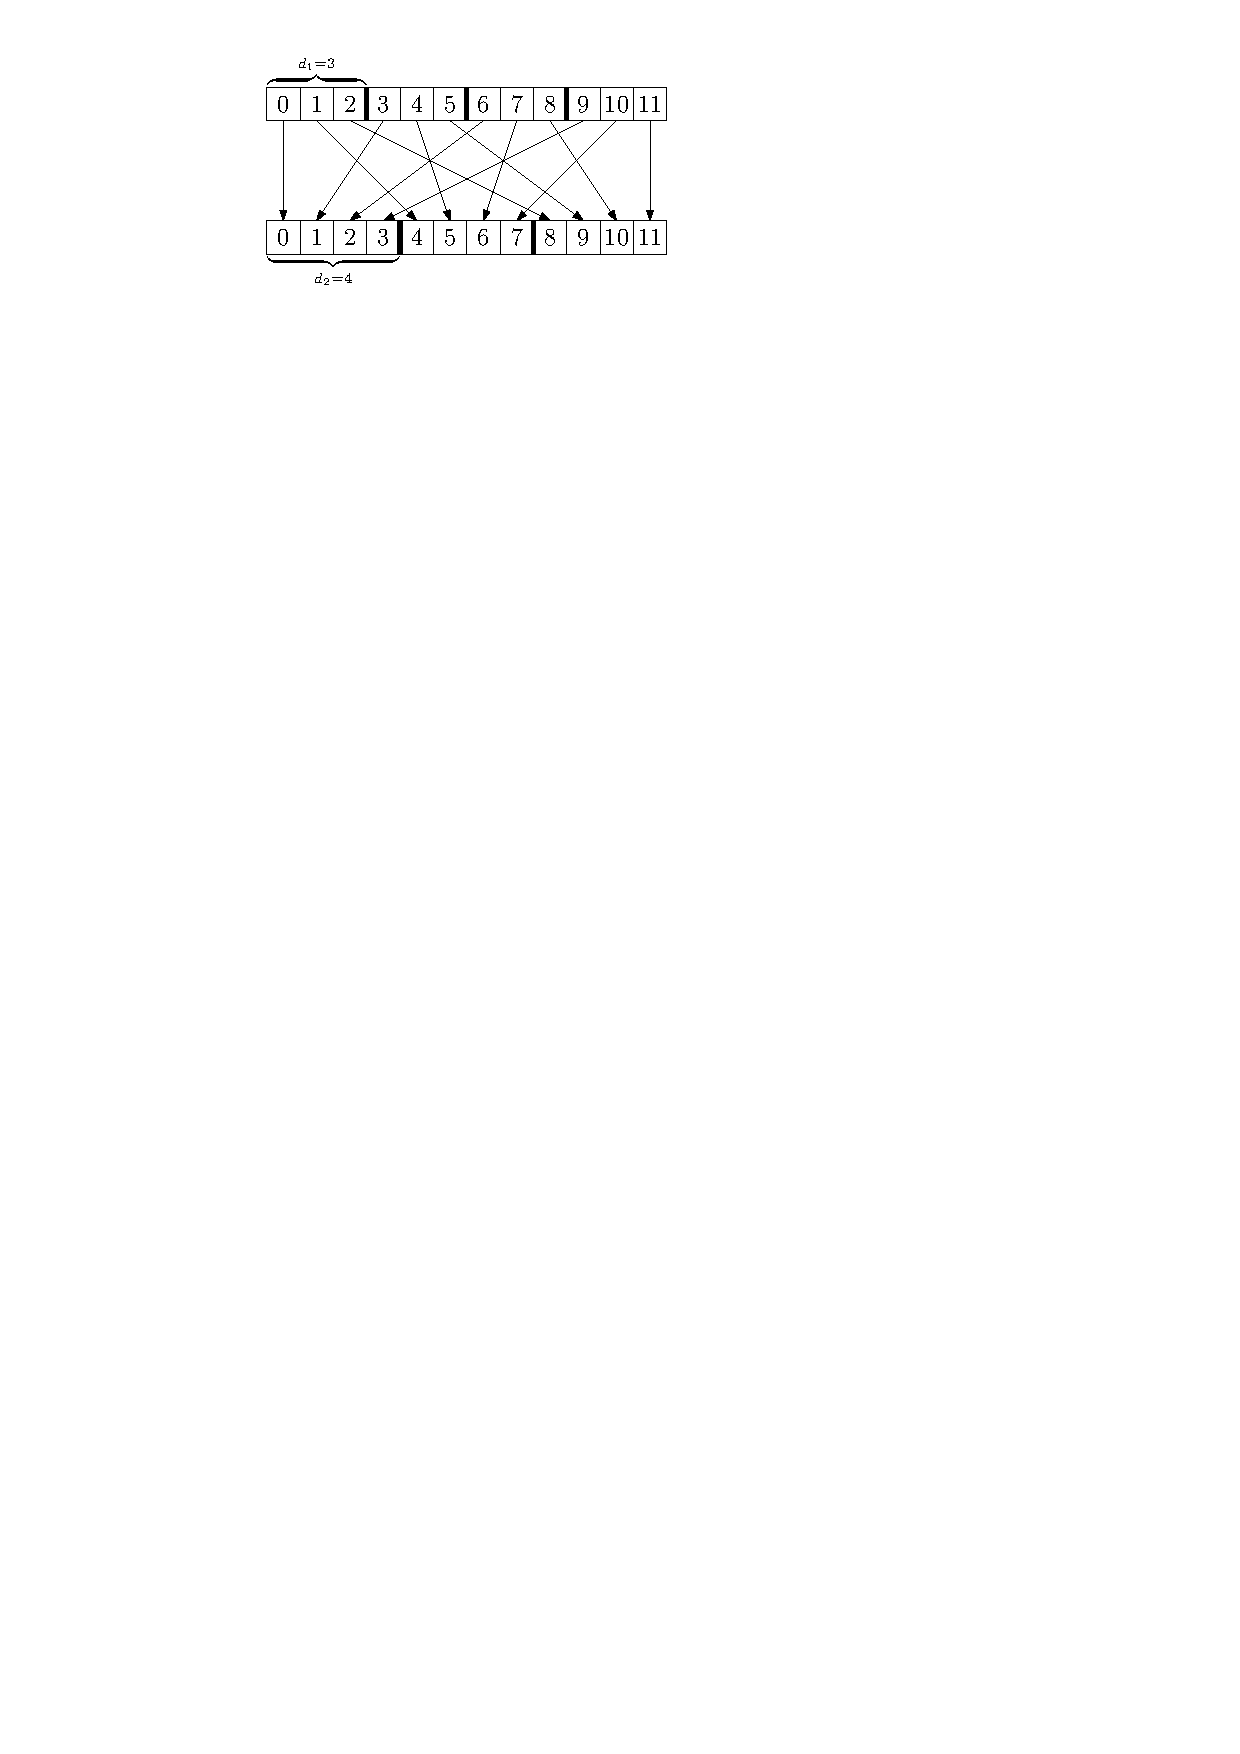
\includegraphics{transpose}
\caption{Illustration of the \texttt{transpose} operation}
\label{fig:transpose}
\end{figure}

Since this operation changes the order of the elements, the basic
dependency tracking does not work anymore: As you can see in
Fig.~\ref{fig:transpose}, the leftmost elements depend on elements from
all over the source array. To track these dependencies correctly, the
implementation of \texttt{sliceJobs} in \texttt{FAJob} must be
fundamentally different. In the 
basic case, it returns the smallest single job that still spans all
the requested elements. However, in the \texttt{transpose} case, this
would (almost)
always be the root job, and hence split dependency tracking would
be useless. Therefore,
in the \texttt{transpose} case, the \texttt{sliceJobs} method will
return multiple jobs: it exhaustively searches through the job-tree
and only returns the jobs at the bottom of the split-tree (i.e. jobs
that actually calculate something) responsible for calculating the
given elements.

It seems obvious, that how exactly the splitting is done has a
tremendous 
impact on ``how non-blocking'' this operation will end up to be. The
current implementation only tracks dependencies, but does not try to
optimize splitting depending on the exact transpose operation that
should be carried out. Further, it might be an advantage to expose the
transpose operation as a view rather than copying the data. This would
require something like a ``dependency mapper'' to convert dependency
tracking between the view and the underlying structure.

Another idea is to make the \texttt{FlowArray} structure inherently aware of
the two dimensions and do the splitting in surfaces (or cubes for
three dimensions) instead of intervals only. This could lead to better
alignment but will certainly lead to a more complex implementation and
difficulties in integrating with the typing system.

\section{Evaluation}
\label{sec:evaluation}

\subsection{Setup}

We have tested the performance of \texttt{FlowArrays} against
\texttt{ParArrays} by calculating the scalar product of two vectors. Refer to
Fig.~\ref{fig:scalar-product} for the implementation of the
benchmark. You'll notice the operations \texttt{zipMap} and
\texttt{zipMapFold}: These are consolidated operations that use the
\texttt{FAJob} structure but do not store intermediate results. As we
will see, they greatly improve performance. Refer to
Fig.~\ref{fig:zipmapfold-semeq} for semantic equivalences of these
operations. 

\begin{figure}
\begin{alltt}{\scriptsize
x.zipMap(y)(f)             <-->  x.zip(y).map(f.tupled)
x.zipMapFold(y)(f)(z)(g)   <-->  x.zip(y).map(f.tupled).fold(z)(g)}
\end{alltt}
\caption{Semantic equivalences for \texttt{zipMap} and
  \texttt{zipMapFold}}
\label{fig:zipmapfold-semeq}
\end{figure}

\begin{figure}
\begin{minipage}[t]{6cm}
\begin{alltt}
{\scriptsize
val x = FlowArray.tabulate(size)(x => x*x)
val y = FlowArray.tabulate(size)(x => x*x)

(x zip y).map(x => x._1 * x._2).fold(0)(_ + _).blocking
// OR
(x zipMap y)(_ * _).fold(0)(_ + _).blocking
// OR
(x zipMapFold y)(_ * _)(0)(_ + _).blocking
}
\end{alltt}
\end{minipage}
\caption{Implementation of scalar product with \texttt{FlowArrays}}
\label{fig:scalar-product}
\end{figure}

We have varied the size of the two vectors from $8 \cdot 10^6$ to $13
\cdot 10^6$ elements with full parallelization. Further, we have
tested the scalability by setting the parallelism level to $1,2$ and
$4$ for \texttt{FlowArrays} (\texttt{ParArrays} have only been measured with full
parallelism). The metrics we collected were the execution time and the
garbage collection time (sum of all non-final GC runtimes).

The benchmarks have been executed on a Intel i7-2620M with java
version 1.7.0\_04, Java(TM) SE Runtime Environment (build
1.7.0\_04-b20), Java HotSpot(TM) 64-Bit Server VM (build 23.0-b21,
mixed mode). The exact java command used is \texttt{java -Xmx2048m
  -Xms2048m -XX:+UseCondCardMark -verbose:gc -XX:+PrintGCDetails
  -server <classname>}.

\subsection{Results}

Please refer to Fig.~\ref{fig:par-bench} and Fig.~\ref{fig:size-bench}
for the 
results of the benchmarks. In both figures, we show the total
execution time, the time spent in garbage collection and the
``normalized execution time'', i.e. the total time minus the time
spent in garbage collection.

The time in garbage collection is the sum of the runtimes of all minor
GC cycles. No full GC cycles have been performed during the
benchmarks. Please note that the GC time is an approximation (minor GC
cycles can run in parallel) and hence the ``normalized execution
time'' may become negative.

\begin{figure}
\subfigure[Execution Time]{\plot{par-time}}
\subfigure[GC Time]{\plot{par-gctime}}
\subfigure[Normalized Time]{\plot{par-ntime}}
\caption{Parallelization benchmarks of scalar product ($size = 10^7$)}
\label{fig:par-bench}
\end{figure}

\begin{figure}
\subfigure[Execution Time]{\plot{size-time}}
\subfigure[GC Time]{\plot{size-gctime}}
\subfigure[Normalized Time]{\plot{size-ntime}}
\caption{Size benchmarks of scalar product ($P = 4$)}
\label{fig:size-bench}
\end{figure}

\subsection{Interpretation}
First of all we must notice the huge overhead that garbage collection
brings, especially for the benchmark using the simple \texttt{zip},
\texttt{map} and \texttt{fold} operations, against which the actual
calculation time becomes negligible. This 
is already strong evidence, that intermediate results should be
avoided (as is done in \texttt{zipMap} and \texttt{zipMapFold}).

Further note that octave \cite{eaton1997gnu} takes around $290 ms$ for
the same calculation on the same machine, we can hence say the
execution times (when disregarding garbage collection) are
comparable.

Other benchmarks for matrix multiplication that have been written but
not 
yet been thoroughly run, have already indicated that garbage
collection might take a big amount of time during calculation.

We come to the conclusion, that allocating memory for and
storing results of small, intermediate steps seems to be a severe
performance 
killer. When continuing in the flow approach, means of reducing
intermediate storage steps (such as the
\texttt{zipMap} and the \texttt{zipMapFold} operations) will need to
be considered as they greatly increase performance. If the \texttt{FlowArray}
framework is able to do conversions like \texttt{zip}, \texttt{map}
$\to$ \texttt{zipMap} automatically, huge performance may be gained
without any additional effort from the programmer using the \texttt{FlowArrays}.

\section{Conclusion}
\label{sec:conclusion}

We have designed and implemented a fixed-size version of a non-blocking
\texttt{ParArray} like datastructure -- the \texttt{FlowArray} -- and succeeded in
implementing all operations necessary to represent matrix
multiplication in the programming model.

Our benchmarks suggest that garbage collection due to full
intermediate result creation (especially for operations like
\texttt{zip}) impact performance negatively and that having
consolidated operations (such as \texttt{zipMap}) removes a lot of
this overhead.

The data hence shows that avoiding storage of intermediate elements in
a dataflow graph significantly speeds up the whole calculation due to the fewer
allocated memory and hence the reduced garbage collection time.

Therefore, it is our proposition, to extend \texttt{FlowArrays} to do such
reductions (like \texttt{zip}, \texttt{map} $\to$ \texttt{zipMap})
automatically, before the calculation is started. With automatically
we mean either through static analysis -- which would also benefit
datastructures of smaller size -- or dynamically at runtime using
views and invoking calculation as necessary. Which approach is more
promising needs to be evaluated using real-life code samples.

It is however important to note, that the latter approach requires a
flow based programming model: a \texttt{ParArray} (or any other imperative,
blocking structure) is unable to consolidate calculation steps at
runtime, as it is required to finish calculation before the call may
be returned and hence no lazily calculated views may exist, which in
turn entirely prevents reduction of calculation steps.

\bibliographystyle{abbrv}
\bibliography{bib}

\end{document}

%%% Local Variables: 
%%% mode: latex
%%% TeX-master: t
%%% End: 
